
\documentclass[10pt,letterpaper]{article}
\usepackage[top=0.85in,left=2.75in,footskip=0.75in]{geometry}

% amsmath and amssymb packages, useful for mathematical formulas and symbols
\usepackage{amsmath,amssymb}

% Use adjustwidth environment to exceed column width (see example table in text)
\usepackage{changepage}

% textcomp package and marvosym package for additional characters
\usepackage{textcomp,marvosym}

% cite package, to clean up citations in the main text. Do not remove.
\usepackage{cite}

% Use nameref to cite supporting information files (see Supporting Information section for more info)
\usepackage{nameref,hyperref}

% line numbers
\usepackage[right]{lineno}

% ligatures disabled
\usepackage[nopatch=eqnum]{microtype}
\DisableLigatures[f]{encoding = *, family = * }

% color can be used to apply background shading to table cells only
%\usepackage[table]{xcolor}

% array package and thick rules for tables
\usepackage{array}

% create "+" rule type for thick vertical lines
\newcolumntype{+}{!{\vrule width 2pt}}

% create \thickcline for thick horizontal lines of variable length
\newlength\savedwidth
\newcommand\thickcline[1]{%
  \noalign{\global\savedwidth\arrayrulewidth\global\arrayrulewidth 2pt}%
  \cline{#1}%
  \noalign{\vskip\arrayrulewidth}%
  \noalign{\global\arrayrulewidth\savedwidth}%
}

% \thickhline command for thick horizontal lines that span the table
\newcommand\thickhline{\noalign{\global\savedwidth\arrayrulewidth\global\arrayrulewidth 2pt}%
\hline
\noalign{\global\arrayrulewidth\savedwidth}}


% Remove comment for double spacing
%\usepackage{setspace} 
%\doublespacing

% Text layout
\raggedright
\setlength{\parindent}{0.5cm}
\textwidth 5.25in 
\textheight 8.75in

% Bold the 'Fig #' in the caption and separate it from the title/caption with a period
% Captions will be left justified
\usepackage[aboveskip=1pt,labelfont=bf,labelsep=period,justification=raggedright,singlelinecheck=off]{caption}
\renewcommand{\figurename}{Fig}

% Use the PLoS provided BiBTeX style
\bibliographystyle{plos2015}

% Remove brackets from numbering in List of References
\makeatletter
\renewcommand{\@biblabel}[1]{\quad#1.}
\makeatother



% Header and Footer with logo
\usepackage{lastpage,fancyhdr,graphicx}
\usepackage{epstopdf}
\usepackage{lmodern}
%\pagestyle{myheadings}
\pagestyle{fancy}
\fancyhf{}
%\setlength{\headheight}{27.023pt}
%\lhead{\includegraphics[width=2.0in]{PLOS-submission.eps}}
\rfoot{\thepage/\pageref{LastPage}}
\renewcommand{\headrulewidth}{0pt}
\renewcommand{\footrule}{\hrule height 2pt \vspace{2mm}}
\fancyheadoffset[L]{2.25in}
\fancyfootoffset[L]{2.25in}
\lfoot{\today}

%% Include all macros below

\newcommand{\lorem}{{\bf LOREM}}
\newcommand{\ipsum}{{\bf IPSUM}}

%% END MACROS SECTION

%% personal packages and macro
%%% packages
\usepackage[utf8]{inputenc}        % allow utf-8 input
\usepackage[T1]{fontenc}           % use 8-bit T1 fonts
\usepackage[dvipsnames, table]{xcolor}
\usepackage{tabularx}
\usepackage{multirow}
\usepackage{pifont}
\usepackage{csvsimple}
\usepackage[font={small},textfont={it},labelfont={bf}]{caption}
\usepackage{subcaption}
\usepackage{graphicx}
\usepackage{url}                   % simple URL typesetting
\usepackage{booktabs}              % professional-quality tables
\usepackage{makecell}
\usepackage{amsfonts}              % blackboard math symbols
\usepackage{amsmath}
\usepackage{nicefrac}              % compact symbols for 1/2, etc.
\usepackage{microtype}             % microtypography
\usepackage{enumitem}
\usepackage[export]{adjustbox}


%not compatible with cite package
%\usepackage[natbib=true,style=nature,maxnames=999,maxcitenames=2,backend=biber]{biblatex}
%\addbibresource{references.bib}

%%% macros
\DeclareMathOperator*{\argmin}{arg\,min}
\newcommand{\indep}{\perp \!\!\! \perp}
\newtheorem{assumption}{Assumption}

\definecolor{dark_blue}{rgb}{0,0,.65}
\definecolor{dark_green}{rgb}{0,.5,.15}

\hypersetup{pdftex,  % needed for pdflatex
  breaklinks=true,  % so long urls are correctly broken across lines
  colorlinks=true,
  linkcolor=dark_blue,
  citecolor=dark_green,
}
\colorlet{P}{ForestGreen}
\colorlet{I}{MidnightBlue}
\colorlet{C}{YellowOrange}
\colorlet{O}{DarkOrchid}
\colorlet{T}{Gray}



\begin{document}
\vspace*{0.2in}

\section*{Supporting information}

\paragraph*{S4 Fig.}
\label{apd:causal_variables}
{\bf Types of causal variables.}

Fig \ref{fig:causal_variables} illustrates the different types of causal variables.

\begin{figure}[h!]
    \begin{minipage}[t]{0.32\linewidth}
        \centering
        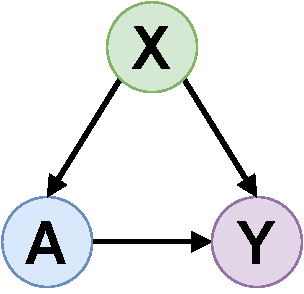
\includegraphics[width=0.72\linewidth]{img_supp_final/confounder.pdf}
        \small\sffamily Confounder
    \end{minipage}
    \hfill
    \begin{minipage}[t]{0.32\linewidth}
        \centering
        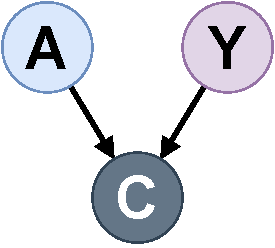
\includegraphics[width=0.72\linewidth]{img_supp_final/collider.pdf}
        \small\sffamily Collider
    \end{minipage}
    \hfill
    \begin{minipage}[t]{0.32\linewidth}
        \centering
        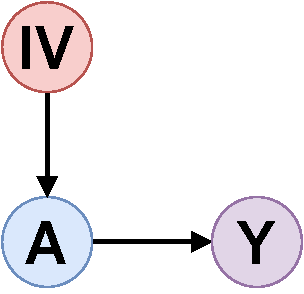
\includegraphics[width=0.72\linewidth]{img_supp_final/instrumental_variable.pdf}
        \small\sffamily Instrumental \\variable
    \end{minipage}
    \vfill
    \begin{minipage}[t]{0.4\linewidth}
        \centering
        
\includegraphics[width=.9\linewidth]{img_supp_final/mediator.pdf}%
        \\
        \small\sffamily Mediator
    \end{minipage}
    \hfill
    \begin{minipage}[t]{0.4\linewidth}
        \centering
        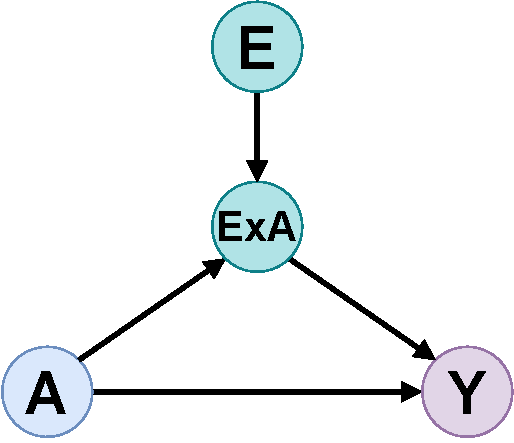
\includegraphics[width=\linewidth]{img_supp_final/effect_modifier.pdf}%
        % \llap{%
        %   \raisebox{.555\linewidth}{\colorbox{black!10}{\parbox{1.9\linewidth}{%
        %         \sffamily\small\hspace*{-1.3ex}%
        %         \begin{tabular}{r@{\hskip 1ex}lr@{\hskip 1ex}l}
        %           A:  & Treatment                    & Y: & Outcome         \\
        %           X:  & Confounder                   & C: & Collider        \\
        %           IV: & Instrumental va\rlap{riable}                        \\
        %           M:  & Mediator                     & E: & Effect modifier \\
        %         \end{tabular}%
        %         \vspace*{-.3ex}
        %       }}\hspace*{.84\linewidth}%
        %   }}
        \small\sffamily Effect modifier \scriptsize\\Represented
        following \cite{attia2022proposal}
    \end{minipage}
    \caption{\textbf{The five categories of causal variables needed for our framework.}\\ A:
        Treatment, X: Confounder, IV: Instrumental variable, M: mediator, Y:
        Outcome, C: Collider, E: Effect modifier.}\label{fig:causal_variables}
\end{figure}


\bibliography{references}


\end{document}
